\documentclass{article}
\usepackage[T1]{fontenc}
\usepackage[utf8]{inputenc}
\usepackage[a4paper, total={6in, 11in}]{geometry}
\usepackage{algorithm}
\usepackage{amsfonts}
\usepackage{algpseudocode}
\usepackage{float}
\usepackage{graphicx}
\usepackage{subcaption}
\usepackage{amsmath}

\def\v{0.47}

\title{%
	Obliczenia naukowe \\
	\large Lista 4}
\author{Szymon Janiak}
\begin{document}
\maketitle

\section*{Zadanie 1}
\subsection*{Opis problemu}
	Napisać funkcję obliczającą ilorazy różnicowe dla podanych węzłów oraz wartości danej funkcji w tych węzłach.
\subsection*{Dane wejściowe}\label{1.in-data}
	\begin{itemize}
		\item \texttt{x} — wektor długości $n + 1$ zawierający węzły $x_0 ,\dots ,x_n$
		\item \texttt{f} — wektor długości $n + 1$ zawierający wartości interpolowanej funkcji w węzłach $f(x_0), \dots, f(x_n)$
	\end{itemize}
\subsection*{Dane wyjściowe}
	\begin{itemize}
	    \item \texttt{fx} — wektor długości $n + 1$ zawierający obliczone ilorazy różnicowe
	\end{itemize}
\subsection*{Rozwiązanie}
	\begin{algorithm}
	\caption{Obliczanie ilorazów różnicowych}
	\begin{algorithmic}[1]
	    \Function{DifferenceQuotients}{$x, f$}
	        \State $fx \gets []$
	        \State $f\_copy \gets \text{copy}(f)$
	        \State $\text{len} \gets \text{length}(x)$
	        
	        \For{$i \gets 1$ \textbf{to} $\text{len}$}
	            \For{$k \gets (i - 1)$ \textbf{downto} $1$}
	                \State $a \gets f\_copy[k + 1] - f\_copy[k]$
	                \State $b \gets (x[i] - x[k])$
	                \State $f\_copy[k] \gets \frac{a}{b}$
	            \EndFor
	            \State $\text{push!}(fx, f\_copy[1])$
	        \EndFor
	        
	        \State \textbf{return} $fx$
	    \EndFunction
	\end{algorithmic}
	\end{algorithm}
\subsection*{Opis użytego algorytmu}
	Do działania naszego algorytmu tworzymy kopię wartości $fx$, w której będziemy obliczać kolejne iteracje naszego algorytmu. Dla oszczędności wykorzystywanej pamięci będziemy zapamiętywać jedynie ostatnio obliczone wartości, gdyż tylko takie będą nam potrzebne. Zewnętrzna pętla iteruje po kolejnych węzłach $x_i$, natomiat wewnętrzna oblicza ilorazy różnicowe dla danej iteracji według wzoru:\\
\centerline{$f[x_0, x_1, \ldots, x_k] = \frac{f[x_1, x_2, \ldots, x_k] - f[x_0, x_1, \ldots, x_{k-1}]}{x_k - x_0}$}
	Po zakończeniu obliczeń dla danego $i$ do naszej tablicy wyników dodajemy jedynie pierwszy iloraz różnicowy. Algorytm ten bazuje na obliczaniu ilorazów różnicowych dla coraz to mniejszych zbiorów węzłów.

\clearpage

\section*{Zadanie 2}
\subsection*{Opis problemu}
	Napisać funkcję obliczającą wartość wielomianu interpolacyjnego stopnia $n$ w postaci Newtona $N_n(x)$ w punkcie $x = t$ za pomocą algorytmu uogólnionego Hornera w czasie $O(n)$.
\subsection*{Dane wejściowe}
	\begin{itemize}
	    \item \texttt{x} — wektor długości $n+1$ zawierający węzły $x_0,\dots,x_n$
	    \item \texttt{fx} — wektor długości $n+1$ zawierający ilorazy różnicowe $f[x_0], \dots, f[x_0,\dots,x_n]$
	    \item \texttt{t} — punkt, w którym należy obliczyć wartość wielomianu
	\end{itemize}
\subsection*{Dane wyjściowe}
	\begin{itemize}
	    \item \texttt{nt} — wartość wielomianu w punkcie \texttt{t}
	\end{itemize}
\subsection*{Rozwiązanie}
	\begin{algorithm}
	\caption{Wartość wielomianu Newtona}
	\begin{algorithmic}[1]
	    \Function{NewtonValue}{$x, fx, t$}
	        \State $\text{len} \gets \text{length}(x)$
	        \State $n\_value \gets fx[\text{len}]$
	        
	        \For{$k \gets (\text{len} - 1)$ \textbf{downto} $1$}
	            \State $n\_value \gets n\_value \cdot (t - x[k]) + fx[k]$
	        \EndFor
	        
	        \State \textbf{return} $n\_value$
	    \EndFunction
	\end{algorithmic}
	\end{algorithm}
\subsection*{Opis użytego algorytmu}
	Algorytm bazuje na uogólnionym sposobie Hornera w czasie liniowym. Początkowo ustawiamy naszą wartość na wartość współczynnika o najwyższym stopniu, czyli $f[len]$, gdzie $len$ to liczba węzłów. W każdej iteracji pętli aktualizowana jest wartość według uogólnionego wzoru Hornera:
\centerline{$n(x) = f[x_1] + (x - x_1) \left[f[x_2] + (x - x_2) \left[f[x_3] + \ldots + (x - x_{n-1}) \left[f[x_n]\right]\ldots\right]\right]$}
	Po zakończeniu pętli algorytm zwraca obliczoną wartość, która reprezentuje wartość wielomianu Newtona w punkcie $t$.

\clearpage

\section*{Zadanie 3}
\subsection*{Opis problemu}
	Napisać funkcję obliczającą współczynniki postaci naturalnej wielomianu interpolacyjnego stopnia $n$ w postaci Newtona $N_n(x)$.
\subsection*{Dane wejściowe}
	\begin{itemize}
	    \item \texttt{x} — wektor długości $n+1$ zawierający węzły $x_0,\dots,x_n$
	    \item \texttt{fx} — wektor długości $n+1$ zawierający ilorazy różnicowe $f[x_0], \dots, f[x_0,\dots,x_n]$
	\end{itemize}
\subsection*{Dane wyjściowe}
	\begin{itemize}
	    \item \texttt{a} — wektor długości $n+1$ zawierający obliczone współczynniki postaci naturalnej ($a_n x^n + a_{n-1} x^{n-1} + \cdots a_1 x + a_0$)
	\end{itemize}
\subsection*{Rozwiązanie}
	\begin{algorithm}
	\caption{Obliczanie współczynników naturalnego kształtu wielomianu}
	\begin{algorithmic}[1]
	    \Function{Natural}{$x, fx$}
	        \State $\text{len} \gets \text{length}(x)$
	        \State $f\_copy \gets \text{copy}(fx)$
	        
	        \For{$i \gets (\text{len} - 1)$ \textbf{downto} $1$}
	            \State $f\_copy[i] \gets fx[i] - f\_copy[i + 1] \cdot x[i]$
	            
	            \For{$j \gets (i + 1)$ \textbf{to} $(\text{len} - 1)$}
	                \State $f\_copy[j] \gets f\_copy[j] - f\_copy[j + 1] \cdot x[i]$
	            \EndFor
	        \EndFor
	        
	        \State \textbf{return} $f\_copy$
	    \EndFunction
	\end{algorithmic}
	\end{algorithm}
\subsection*{Opis użytego algorytmu}
	Algorytm ten korzysta z obliczonych ilorazów różnicowych dla wielomianu interpolacyjnego. Ilorazy różnicowe to $c_0, c_1, c_2 \dots c_n$. Współczynnikiem $a_n$ stojącym przy najwyższej potędze, $x^n$ jest $c_n$. Dzięki temu jesteśmy w stanie schodząc do coraz niższych potęg obliczać współczynniki. Każda iteracja wykorzystuje obliczone wcześniej współczynniki w postaci naturalnej, które aktualizuje o nowe potęgi.

\clearpage

\section*{Zadanie 5}
	Przetestować metodę \texttt{draw\_Nnfx} na kilku zadanych poniżej funkcjach.
\subsection*{Wyniki}
	\begin{figure}[H]
	    \centering
		\begin{subfigure}[b]{\v\linewidth}
			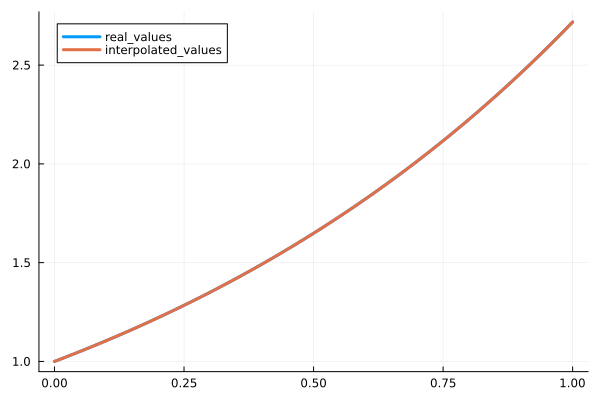
\includegraphics[width=\linewidth]{graphs/zad5.a.5.png}
			\caption{$n = 5$}
		\end{subfigure}
		\begin{subfigure}[b]{\v\linewidth}
			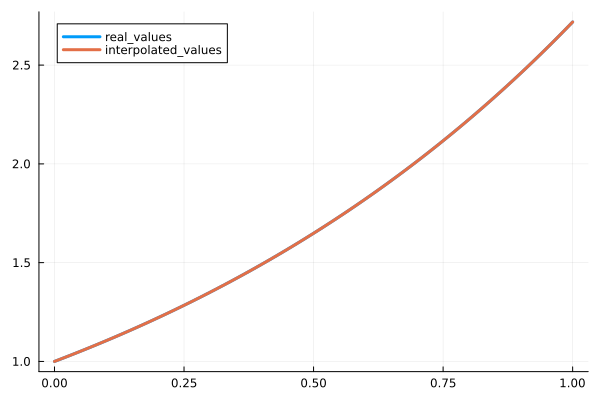
\includegraphics[width=\linewidth]{graphs/zad5.a.10.png}
			\caption{$n = 10$}
		\end{subfigure}
		\begin{subfigure}[b]{\v\linewidth}
			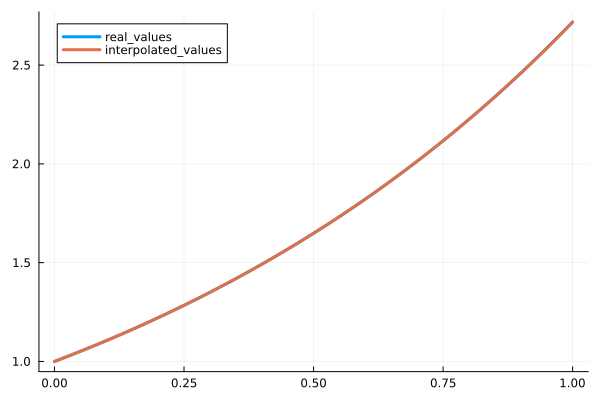
\includegraphics[width=\linewidth]{graphs/zad5.a.15.png}
			\caption{$n = 15$}
		\end{subfigure}
	\\{$f(x) = e^x$ w przedziale $[0;1]$ dla $n = 5,10,15$}
	\end{figure}

	\begin{figure}[H]
	    \centering
		\begin{subfigure}[b]{\v\linewidth}
			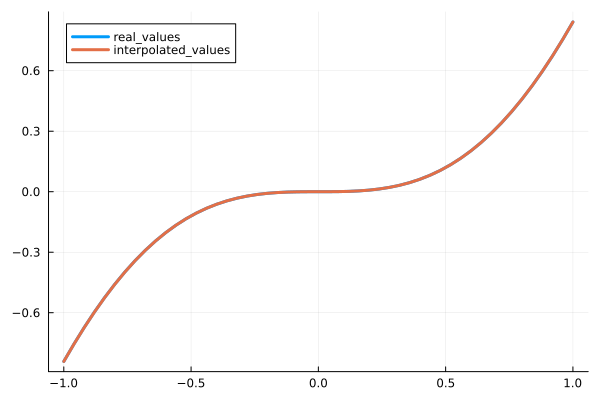
\includegraphics[width=\linewidth]{graphs/zad5.b.5.png}
			\caption{$n = 5$}
		\end{subfigure}
		\begin{subfigure}[b]{\v\linewidth}
			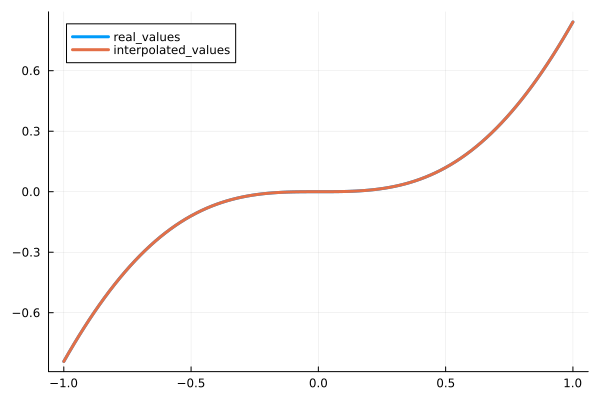
\includegraphics[width=\linewidth]{graphs/zad5.b.10.png}
			\caption{$n = 10$}
		\end{subfigure}
		\begin{subfigure}[b]{\v\linewidth}
			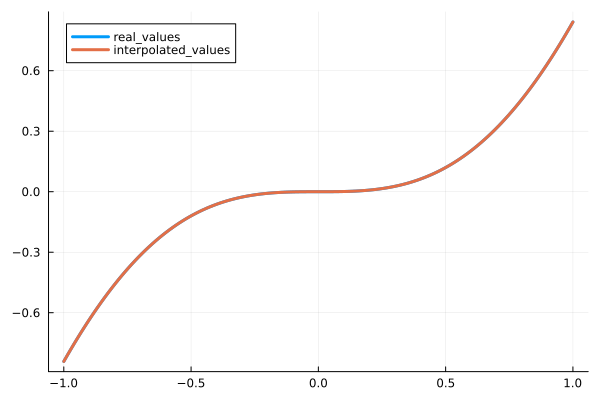
\includegraphics[width=\linewidth]{graphs/zad5.b.15.png}
			\caption{$n = 15$}
		\end{subfigure}
	\\{$f(x) = x^2 \cdot sin x$ w przedziale $[-1;1]$ dla $n = 5,10,15$}
	\end{figure}
\subsection*{Wnioski}
	Na wykresach możemy zauważyć, że wykres interpolowanej przez nas funkcji pokrywa się praktycznie idealnie z rzeczywistymi wartościami dla stopni $n = 5, 10, 15$

\section*{Zadanie 6}
	Przetestować metodę \texttt{draw\_Nnfx} na kilku zadanych poniżej funkcjach.
\subsection*{Wyniki}
	\begin{figure}[H]
	    \centering
		\begin{subfigure}[b]{\v\linewidth}
			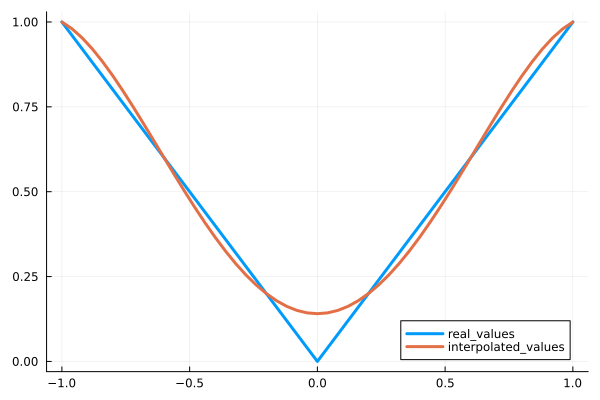
\includegraphics[width=\linewidth]{graphs/zad6.a.5.png}
			\caption{$n = 5$}
		\end{subfigure}
		\begin{subfigure}[b]{\v\linewidth}
			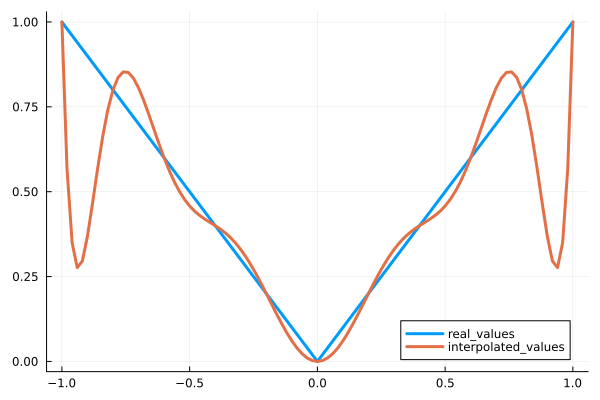
\includegraphics[width=\linewidth]{graphs/zad6.a.10.png}
			\caption{$n = 10$}
		\end{subfigure}
		\begin{subfigure}[b]{\v\linewidth}
			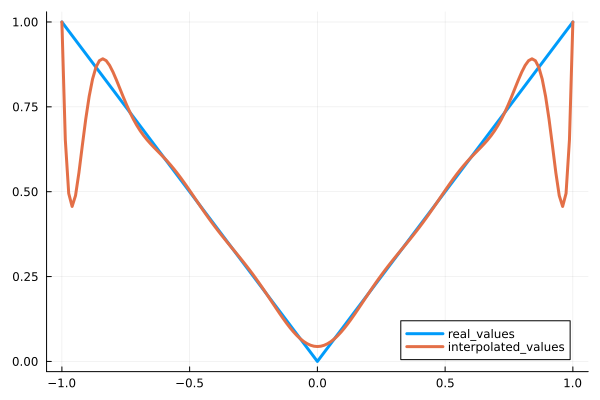
\includegraphics[width=\linewidth]{graphs/zad6.a.15.png}
			\caption{$n = 15$}
		\end{subfigure}
	\\{$f(x) = |x|$ w przedziale $[-1;1]$ dla $n = 5,10,15$}
	\end{figure}

	\begin{figure}[H]
	    \centering
		\begin{subfigure}[b]{\v\linewidth}
			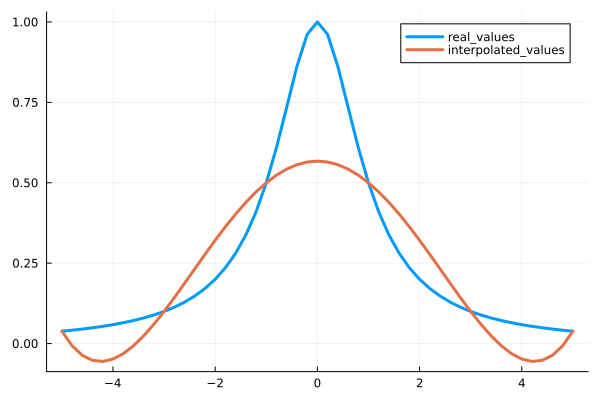
\includegraphics[width=\linewidth]{graphs/zad6.b.5.png}
			\caption{$n = 5$}
		\end{subfigure}
		\begin{subfigure}[b]{\v\linewidth}
			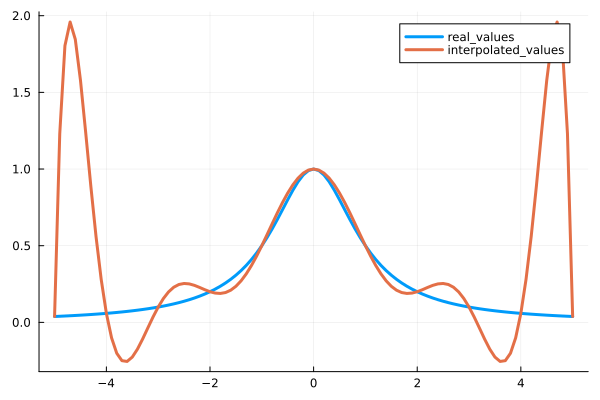
\includegraphics[width=\linewidth]{graphs/zad6.b.10.png}
			\caption{$n = 10$}
		\end{subfigure}
		\begin{subfigure}[b]{\v\linewidth}
			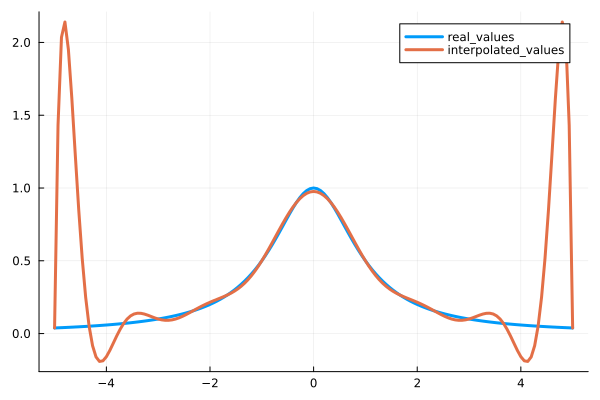
\includegraphics[width=\linewidth]{graphs/zad6.b.15.png}
			\caption{$n = 15$}
		\end{subfigure}
	\\{$f(x) = \frac{1}{1+x^2}$ w przedziale $[-5;5]$ dla $n = 5,10,15$}
	\end{figure}

\clearpage
\subsection*{Wnioski}
	Widzimy, że w tym przypadku funkcje nie interpolują się za dobrze. Nie widać również poprawy przy zwiększaniu stopnia $n$ co daje różne rezultaty. Pokazuje to dobrze ograniczenia interpolacji wielomianowej. Lepsze efekty mogłaby przynieść interpolacja wielomianu poprzez podzielenie go na mniejsze przedziały i lepsze dobranie wartości węzłów interpolacji.

\end{document}